\documentclass[12pt]{article}
\usepackage[a4paper]{geometry}
\usepackage{hyperref}
\usepackage{graphicx}
\usepackage{subcaption}
\usepackage{tikz-qtree}

\renewcommand{\baselinestretch}{1.5} 

\begin{document}

\title{Thesis Proposal}
\author{Hossein Naderi \\supervised by Eric Ruppert}
\maketitle

%\begin{enumerate}
%  \item Importance of implementing shared data structures
%\begin{itemize}
%  \item how it helps developers
%  \item why lock free data structures are better than using locks?
%\end{itemize} 
%  \item  What properties matter for a distributed data structure?
%\begin{itemize}
%  \item Correctness condition: Linearizability definition
%  \item Wait-freeness
%\end{itemize} 
%  \item Previous works on distributed queues: more detailed
%\begin{itemize}
%  \item why we are studying queues
%  \item $p$ factor in time complexity of all previous algorithms
%  \item types of current queues in the literature
%  \item previous impractical universal constructions that use long words
%\end{itemize}
%  \item Our contribution
%\begin{itemize}
%  \item polylogarithmic algorithm with respect to $p$ and $Q$ size of the queue
%\end{itemize}
%  \item Explaining ideas
%\begin{itemize}
%  \item using tournament tree to agree on the linearization order
%  \item double refresh
%  \item how to compute a dequeue response
%  \item how to be sure the number of blocks in the root is related to the size of the queue
%  \item memory management as a goal
%\end{itemize}
%\end{enumerate}

\pagebreak

\section{Introduction}

\paragraph{}
Shared data structures have become an essential field in distributed algorithms research.
We are reaching the physical limits of how many transistors we can place on a CPU core. The industry solution to provide more computational power is to increase the number of cores of the CPU. This is why distributed algorithms have become important. It is not hard to see why multiple processes cannot update sequential data structures designed for one process. For example, consider two processes trying to insert some values into a sequential linked list simultaneously. Processes $p,q$ read the same tail node, $p$ changes the next pointer of the tail node to its new node and after that $q$ does the same. In this run, $p$'s update is overwritten. One solution is to use locks; whenever a process wants to do an update or query on a data structure, the process locks it, and others cannot use it until the lock is released. Using locks has some disadvantages; for example, one process might be slow, and holding a lock for a long time prevents other processes from progressing. Moreover, locks do not allow complete parallelism since only the one process holding the lock can make progress. Our approach is to create a lock-free queue data structure that developers can safely use without the disadvantages of locks. Also there is a common problem in previous shared queues we're going to resolve which make their worst case slow.


The question that may arise is, ``What properties matter for a lock-free data structure?''.
Since executions on a shared data structure are different from sequential ones, the correctness conditions also differ. To prove a concurrent object works perfectly, we have to show it satisfies safety and progress conditions. A \textit{safety condition} tells us that the data structure does not return wrong responses, and a \textit{progress property} requires that operations eventually terminate.

The standard safety condition is called \textit{linearizability}, which ensures that for any concurrent execution on a linearizable object, each operation should appear to take effect instantaneously at some moment between its invocation and response. Figure \ref{fig::goodexample} is an example of execution on a linearizable  queue that is initially empty. The arrow shows time, and each rectangle shows the time between the invocation and the termination of an operation. Since \texttt{Enqueue(A)} and \texttt{Enqueue(B)} are concurrent, \texttt{Enqueue(B)} may or may not take effect before \texttt{Enqueue(A)}. The execution in Figure \ref{fig::badexample} is not linearizable since \texttt{A} has been enqueued before \texttt{B}, so it has to be dequeued first.

\begin{figure}[t]
  \center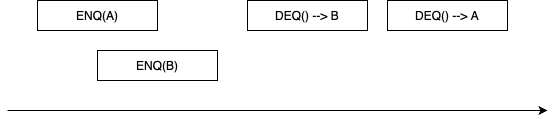
\includegraphics[scale=0.5]{pics/good}
  \caption{\label{fig::goodexample}An example of a linearizable execution. Either \texttt{Enqueue(A)} or \texttt{Enqueue(B)} could take effect first since they are concurrent.}
\end{figure}

\begin{figure}[t]
  \center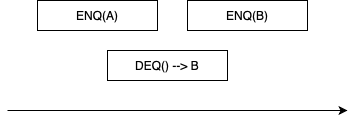
\includegraphics[scale=0.5]{pics/bad}
  \caption{\label{fig::badexample}An example of an execution that is not linearizable. Since \texttt{Enqueue(A)} has completed before \texttt{Enqueue(B)} is invoked the \texttt{Dequeue()} should return \texttt{A}.}
\end{figure}


There are various progress properties; the strongest is wait-freedom, and the more common is lock-freedom. An algorithm is \textit{wait-free} if each operation terminates after a finite number of its own steps. We call an algorithm \textit{lock-free} if, after a sufficient number of steps, one operation terminates. A wait-free algorithm is also lock-free but not vice versa since a lock-free algorithm may terminate after an exponential number of steps.
%From now on, we are going to focus on wait freedom.

%Since executions on a shared data structure are different from sequential ones, the correctness condition also differs. The strongest correctness condition is linearizability, defined as "...". Lock-free is good, but a wait-free algorithm guarantees us every operation terminates after finite steps.

\section{Related Work}
\subsection{List based queues}
In the following paragraphs, we look at previous lock-free queues.
Michael and Scott~\cite{DBLP:conf/podc/MichaelS96} introduced a lock-free queue which we refer to as the MS-queue. A version of it is included in the standard Java Concurrency Package. Their idea is to store the queue elements in a singly-linked list (see Figure~\ref{fig::msq}). Head points to the first node in the linked list that has not been dequeued, and Tail points to the last element in the queue. To insert a node into the linked list, they use atomic primitive operations like \texttt{LL/SC} or \texttt{CAS}. If $p$ processes try to enqueue simultaneously, only one can succeed, and the others have to retry. This makes the amortized number of steps to be $\Omega(p)$ per enqueue. Similarly, dequeue can take $\Omega(p)$ steps.

\begin{figure}[t]
  \center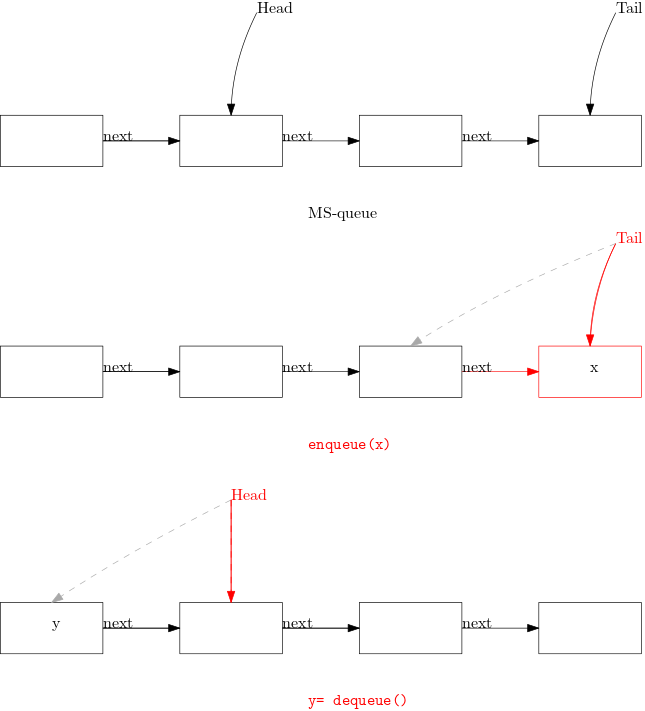
\includegraphics[scale=0.5]{pics/msqueue}
  \caption{\label{fig::msq}MS-queue structure, enqueue and dequeue operations. Red arrow shows new pointer and gray dashed arrow shows the old arrow.}
\end{figure}


Moir, Nussbaum, and Shalev~\cite{DBLP:conf/spaa/MoirNSS05} presented a more sophisticated queue by using the elimination technique. The elimination mechanism has the dual purpose of allowing operations to complete in parallel and reducing contention for the queue. An Elimination Queue consists of an MS-queue augmented with an elimination array. Elimination works by allowing opposing pairs of concurrent operations such as an enqueue and a dequeue to exchange values when the queue is empty or when concurrent operations can be linearized to empty the queue. Their algorithm makes it possible for long-running operations to eliminate an opposing operation. The empirical evaluation showed the throughput of their work is better than MS-queue, but the worst case is still the same; in case there are $p$ concurrent enqueues, their algorithm is not better than MS-queue. 

Hoffman, Shalev, and Shavit~\cite{DBLP:conf/opodis/HoffmanSS07} tried to make the MS-queue more parallel by introducing the Baskets Queue. Their idea is to allow more parallelism by treating the simultaneous enqueue operations as a basket. Each basket has a time interval in which all its nodes' enqueue operations overlap. Since the operations in a basket are concurrent, we can order them in any way. Enqueues in a basket try to find their order in the basket one by one by using \texttt{CAS} operations. However, like the previous algorithms, if there are still $p$ concurrent enqueue operations in a basket, the amortized step complexity remains $\Omega(p)$ per operation.

\begin{figure}[t]
  \center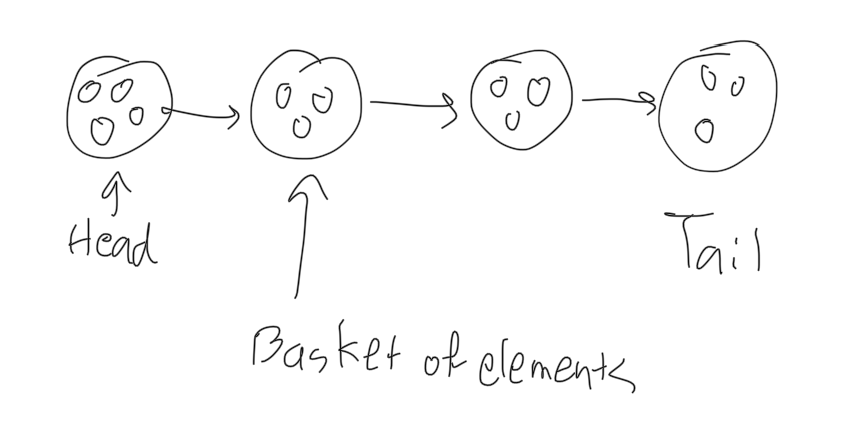
\includegraphics[scale=0.3]{pics/baskets}
  \caption{Baskets queue idea.}
\end{figure}

Ladan-Mozes and Shavit~\cite{DBLP:journals/dc/Ladan-MozesS08} presented an Optimistic Approach to Lock-Free FIFO Queues. They use a doubly-linked list and do fewer \texttt{CAS} operations than MS-queue. But as before, the worst case is when there are $p$ concurrent enqueues which have to be enqueued one by one. The amortized worst-case complexity is still $\Omega(p)$ \texttt{CAS}es.

Hendler et al.~\cite{DBLP:conf/spaa/HendlerIST10} proposed a new paradigm called flat combining. Their queue is linearizable but not lock-free. Their main idea is that with knowledge of all the history of operations, it might be possible to answer queries faster than doing them one by one. In our work we also maintain the whole history. They present experiments that show their algorithm performs well in some situations.

Gidenstam, Sundell and Tsigas~\cite{DBLP:conf/opodis/GidenstamST10} introduced a new algorithm using a linked list of arrays. Global head and tail pointers point to arrays containing the first and last element in the queue and the elements when they are written by \texttt{CAS} operations and dequeued. Their data structure is lock-free. An enqueue or a dequeue searches for the head array or tail array to find the first unmarked element or last written element (see~Figure~\ref{fig::sundell}). Still, if the head array is empty and $p$ processes try to enqueue simultaneously, the step complexity remains $\Omega(p)$.

\begin{figure}[t]
  \center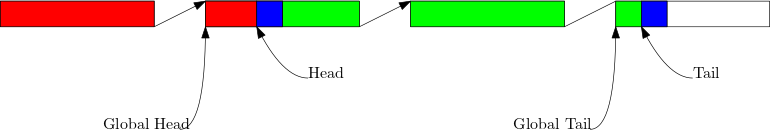
\includegraphics[scale=0.5]{pics/sundell}
    \caption{\label{fig::sundell}Global pointer point to arrays. Head and Tail elements are blue dequeued elements are red and current elements of the queue are in green.}
\end{figure}

Kogan and Petrank~\cite{DBLP:conf/ppopp/KoganP11} introduced wait-free queues based on MS-queue and use Herlihy's helping technique to achieve wait-freedom. Their step complexity is $\Omega(p)$ because of the helping mechanism.

%todo: comparison
%Milman et al.~\cite{DBLP:conf/spaa/MilmanKLLP18} designed BQ: A Lock-Free Queue with Batching. Their idea of batching allows a sequence of operations to be submitted as a batch for later execution. It supports a new notion introduced by the authors called Extended Medium Futures Linearizability.

%Nikolaev and Ravindran~\cite{DBLP:journals/corr/abs-2201-02179} wCQ to be completed.
In the worst-case step complexity of all the list-based queues discussed above, there is a $p$ term that comes from the case all $p$ processes try to do an enqueue simultaneously. Morrison and Afek call this the \textit{CAS retry problem}~\cite{DBLP:conf/ppopp/MorrisonA13}. It is not limited to list-based queues and array-based queues share CAS retry problem as well~\cite{DBLP:conf/spaa/TsigasZ01,DBLP:conf/icdcn/Shafiei09,DBLP:conf/iceccs/ColvinG05} . We are focusing on seeing if we can implement a queue in sublinear steps in terms of $p$ or not.

\subsection{Universal constructions}
Herlihy discussed the possibility of implementing shared objects from other objects~\cite{10.1145/114005.102808}. A \textit{universal construction} is an object that can implement a shared object from any given sequential object. We can implement a concurrent queue using a universal construction. Jayanti proved an $\Omega(\log p)$ lower bound on the worst-case shared-access time complexity of $p$-process universal constructions~\cite{DBLP:conf/podc/Jayanti98a}. He also introduced a construction that achieves $\textsc{O}(\log^2 p)$ shared accesses~\cite{DBLP:conf/podc/ChandraJT98}. His universal construction can be used to create any data structure, but its implementation is not practical because of using unreasonably large-sized \texttt{CAS} operations.

Ellen and Woelfel introduced an implementation of a Fetch\&Inc object with step complexity of log $p$ using $O(\log n$)bit \texttt{LL/SC} objects, where $n$ is the number of operations~\cite{10.1007/978-3-642-41527-2_20}. Their idea has similarities to Jayanti's construction, and they represent the value of the Fetch\&Inc using the history of successful operations. 

%FIFO queues have a wide range of use in OS and applications. The current state-of-the-art queues are implemented using linked lists; that's why they have factor p in their time complexity.

%\href{https://docs.google.com/spreadsheets/d/1cL1tgXXdljkh462sMwkTVMHH_k0MBTmslIVM3xA5VS4/edit#gid=0}{Table of previous works}

%There is a connection between queues and universal constructions. We can implement a universal construction using a queue. We can store operations in the shared queue and compute operations' responses using the queue's content. Some impractical universal constructions are using big words as "...".

\section{Our Contribution}
In this work, we design a queue with $O(\log^2 p +\log q)$ steps per operation, where $q$ is the size of the queue, outperforming queues built by the LinkedList approach. Our idea is similar to Jayanti and Petrovic's multi-enqueuer single-dequeuer Queue~\cite{DBLP:conf/fsttcs/JayantiP05}, but we do not use \texttt{CAS} operations with big words and do not put a limit on the number of concurrent dequeues. We introduce a data structure that allows processes to agree on the linearization ordering of their operations using $\textsc{O}(\log p)$ \texttt{CAS} per operation called a \textit{block tree}. Then we use the block tree as a stepping stone towards our queue algorithm.
A block tree is a tournament tree shared among $p$ processes (see Figure~\ref{fig::blocktree}). Each process has a leaf, and it appends its operations to its leaf. After that, the process tries to propagate its new operation up to the tree's root. An ordering of operations propagated up to a node is stored in that node. All processes agree on the sequence stored in the root and this is used as the linearization ordering. 

\begin{figure}[t]
\begin{center}
\Tree [ [ [ $P_1$ $P_2$ ] [ $P_3$ $P_4$ ] ]
          [ [ $P_5$ $P_6$ ] [ $P_7$ $P_8$ ] ] ]
\end{center}
\caption{ّ\label{fig::blocktree}In the block tree each process has a leaf and in each node there is an ordering of operations stored. Each node tries to propagate its operations up to the root, which stores the final ordering of all operations.}  
\end{figure}

The goal here is to ensure in each propagate step the new operations are propagated up to the parent in $O(\log p)$ steps (see~Figure~\ref{fig::propagstep}). Then, a dequeue operation uses the linearization ordering to compute its answer.


In each propagate step, our algorithm uses a subroutine \textsc{Refresh}($n$) that aggregates new operations from node $n$'s children (that have not already been propagated to $n$) and tries to append them into $n$ using a\texttt{CAS} operation. The general idea is that if we call \textsc{Refresh}($n$) twice, the operations in \texttt{n}'s children before the first \textsc{Refresh}($n$) are guaranteed to be in $n$.
%Since there is a successful instance of \textsc{Refresh}($n$) after the first \textsc{Refresh}($n$), which has appended the talked operations.
Instead of storing operations explicitly in the nodes, we only keep track of the number of them. This allows us to \texttt{CAS} fixed-size objects in each \textsc{Refresh}($n$). To do that, we introduce blocks that only contain the number of operations from the left and the right child in a \textsc{Refresh}() procedure and only propagate the block of the new operations.


\begin{figure}[t]
\begin{center}
\begin{subfigure}[b]{.49\textwidth}
  \centering
  \resizebox{\columnwidth}{!}{
  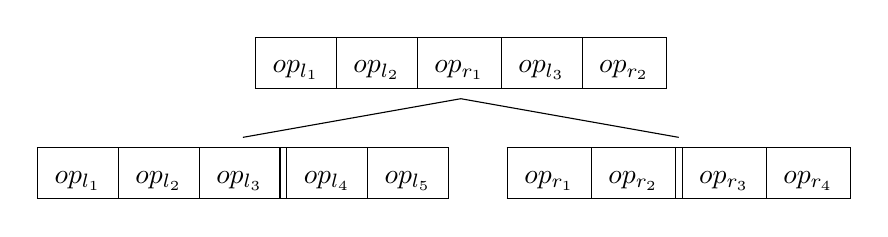
\begin{tikzpicture}[level 1/.style={level distance=1.4cm,sibling distance=0.5cm}]
\Tree [.{\begin{tabular}{|c|c|c|c|c|c|}  \hline $op_{l_1}$ & $op_{l_2}$ & $op_{r_1}$ & $op_{l_3}$ & $op_{r_2}$ \\ \hline \end{tabular}}
{\begin{tabular}{|c|c|c||c|c|}  \hline $op_{l_1}$ & $op_{l_2}$ & $op_{l_3}$ & $op_{l_4}$ & $op_{l_5}$ \\ \hline \end{tabular}}
{\begin{tabular}{|c|c||c|c|}  \hline $op_{r_1}$ & $op_{r_2}$ & $op_{r_3}$ & $op_{r_4}$\\ \hline \end{tabular}} ]
\end{tikzpicture}}
  \caption{Operations after $||$ are new.}
\end{subfigure}
\hfill
\begin{subfigure}[b]{.49\textwidth}
  \centering
  \resizebox{\columnwidth}{!}{
  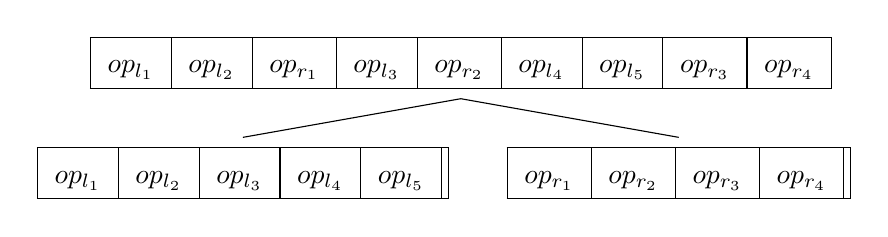
\begin{tikzpicture}[level 1/.style={level distance=1.4cm,sibling distance=0.5cm}]
\Tree [.{\begin{tabular}{|c|c|c|c|c|c|c|c|c|c|}  \hline $op_{l_1}$ & $op_{l_2}$ & $op_{r_1}$ & $op_{l_3}$ & $op_{r_2}$ & $op_{l_4}$ & $op_{l_5}$ & $op_{r_3}$ & $op_{r_4}$  \\ \hline \end{tabular}}
{\begin{tabular}{|c|c|c|c|c||}  \hline $op_{l_1}$ & $op_{l_2}$ & $op_{l_3}$ & $op_{l_4}$ & $op_{l_5}$ \\ \hline \end{tabular}}
{\begin{tabular}{|c|c|c|c||}  \hline $op_{r_1}$ & $op_{r_2}$ & $op_{r_3}$ & $op_{r_4}$\\ \hline \end{tabular}} ]
\end{tikzpicture}}
  \caption{New operations are added to the parent node.}
\end{subfigure}
\caption{\label{fig::propagstep} Successful \texttt{Refresh}, operations in children after $||$ are new.}
\end{center}
\end{figure}

We also implement methods \texttt{Get(i)}, \texttt{Index(op)} to get the $i$th propagated operation and compute the rank of a propagated operation in the linearization. \texttt{Get(i)} finds the block containing the $i$th operation in the root and then finds its sub-block recursively to reach a leaf. \texttt{Index()} is  similar but more complicated, finding super-blocks from a leaf to the root. The main challenge in each level of \texttt{Get(i)} and \texttt{Index(op)} is that it should take polylogarithmic steps with respect to $p$. After appending operations to the root, processes can find out information about the linearization ordering using \texttt{Get(i)} and \texttt{Index(op)}. Now we can implement Enqueue and Dequeue using our block tree. An \texttt{Enqueue(e)} appends an operation with input argument \texttt{e} in the block tree. To do a \texttt{Dequeue()}, first process $p$ first appends a \texttt{DEQ} operation to the tree. Then $p$ finds the rank of the \texttt{DEQ} using \texttt{Index()}, using the rank of the \texttt{DEQ} and the information stored in the root about the queue $p$ computes the rank of  the \texttt{ENQ} having the answer of the \texttt{DEQ}. Finally $p$ returns the argument of that \texttt{ENQ} using \texttt{Get(i)}.

\texttt{Get()} and \texttt{Index()} search among blocks in each level of the tree to find the sub-block or super-block containing the given operation. Each block stores a constant amount of information (like prefix sums) to allow binary searches to find the required block in a node quickly.

The algorithm works as a queue, but \texttt{Get(i)}  may take a long time since it has to find the block containing the $i$th operation at the root level. We came up with a garbage collection only for the root level to reduce the time to find this block to $O(\log q)$. The main idea is to remove a block after its operations are no longer needed. We will store the blocks in the root in a persistent red-black tree to be able only to maintain the remaining information of the queue. It is possible to search in persistent red-black trees with size $n$ in $O(\log n)$ steps and split the tree by a key in $O(\log n)$ steps.  Finally, the algorithm works in $O(\log^2 p +\log q)$ steps.

\section{Next steps}
The current algorithm only works as a queue, but other data structures like stacks share similarities. It might be possible to come up with a generalization for all these types. We have not yet considered space usage, and we use infinite-sized arrays that are not practical. Our future work is to manage the memory of the tree and make it practical.

\section{Planning}
The plan is to finish the writing of the thesis by August 2021. The thesis will contain:
\begin{itemize}
  \item More detailed discussion of previous work
  \item Description of the algorithm, layer by layer
  \item Pseudocode of the algorithm
  \item Proof of linearizability and time analysis
\end{itemize}

We expect to submit a paper of our work to \textit{36th International Symposium on Distributed Computing
October 25-27, 2022, Augusta, Georgia, USA} by May 13.

\bibliography{main} 
\bibliographystyle{ieeetr}

\end{document}
